\documentclass[11pt,a4paper]{report}

\usepackage[utf8]{inputenc}
\usepackage{amsmath}
\usepackage{amsfonts}
\usepackage{subcaption}
\usepackage{amssymb}
\usepackage{graphicx}
\usepackage[left=2cm,right=2cm,top=2cm,bottom=2cm]{geometry}
\usepackage{amsmath}
\usepackage{wrapfig}

\title{ARPA: Autonomous Robotic Pointer Arm}
\author{Helgerud, Erlend \and Håland, André}

\begin{document}
	\maketitle
	\tableofcontents
	\newpage

	%\section{Abstract}
	%\section{Introduction}
	%\section{Related works}
	\section{System description}
	
	\subsection{Architecture}
	The idea of ARPA is to have a 1:1 relationship between a physical robotic arm, and a simulated model in Gazebo. This means that the model in Gazebo should contain (as good as) the same measurements as the physical robot. They will also receive the same control signals leading to synchronized movement. Figure \ref{fig:architecture} show this relationship between the real world and the simulated world.
	
	\begin{figure}[ht]
		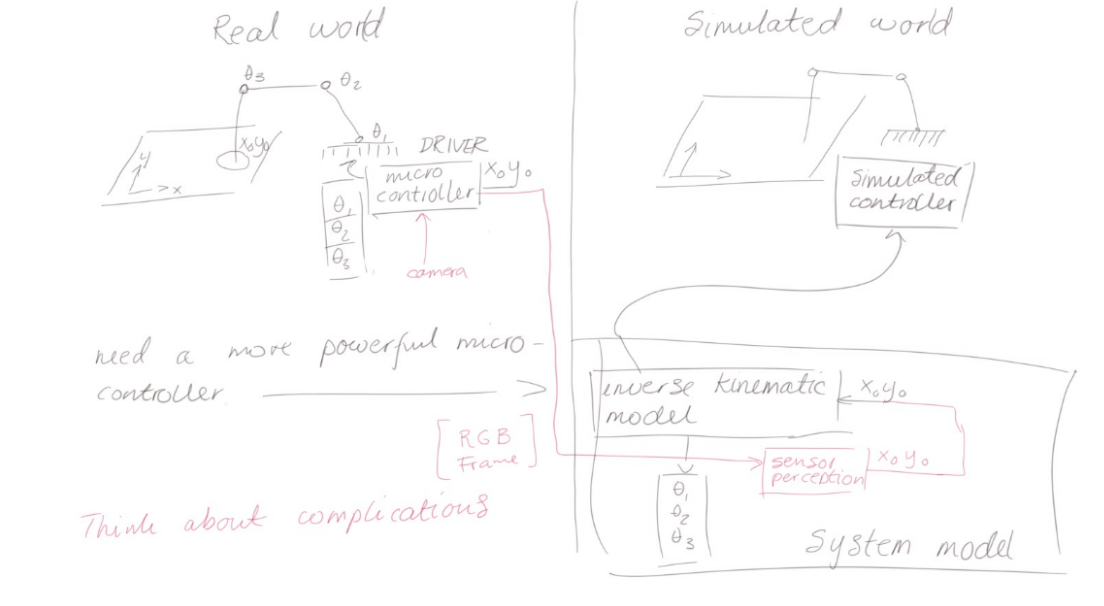
\includegraphics[width=\linewidth]{../Diagrams/Architecture.png}
		\caption{System architecture}
		\label{fig:architecture}
	\end{figure}
	
	
	ARPA is divided into nodes. These nodes each has its own tasks and communicate with each other on different topics to exchange information. Figure \ref{fig:nodegraph} shows the nodes of ARPA, and the topics they communicate on. A circle represents a node, whilst a rectangle represents a topic. The controller node is the center of all actions. It handles the interface between the camera, MATLAB, the physical robotic arm and the model in gazebo. The camera node  sends a Cartesian point in space to the controller. The MATLAB node handles inverse kinematics. It receives Cartesian coordinates from the controller, and sends back five joint angles. The 5DOF Robot node controls the physical robotic arm by writing received angles to the servo motors. The Gazebo node listens to the same topics as 5DOF Robot, and will simulate a robotic model with a 1:1 relationship with the physical arm.
	
As described in \textbf{todo: refer to XX}, we had some challenges with finding the inverse kinematics and have to depend on the Robotics System Toolbox from MATLAB. When running MATLAB as a ROS node, we discovered that it ran quite slowly together with Gazebo. For this reason, we decided to run the ROS network over two computers to separate computing power. This is done by setting a couple of environmental variables in every terminal that uses ROS. Two shell scripts were made for this, and can be sourced to achieve the distributed ROS network. The different colored nodes in figure \ref{fig:nodegraph} represents which computer the node runs on.
	
	\begin{figure}[ht]
		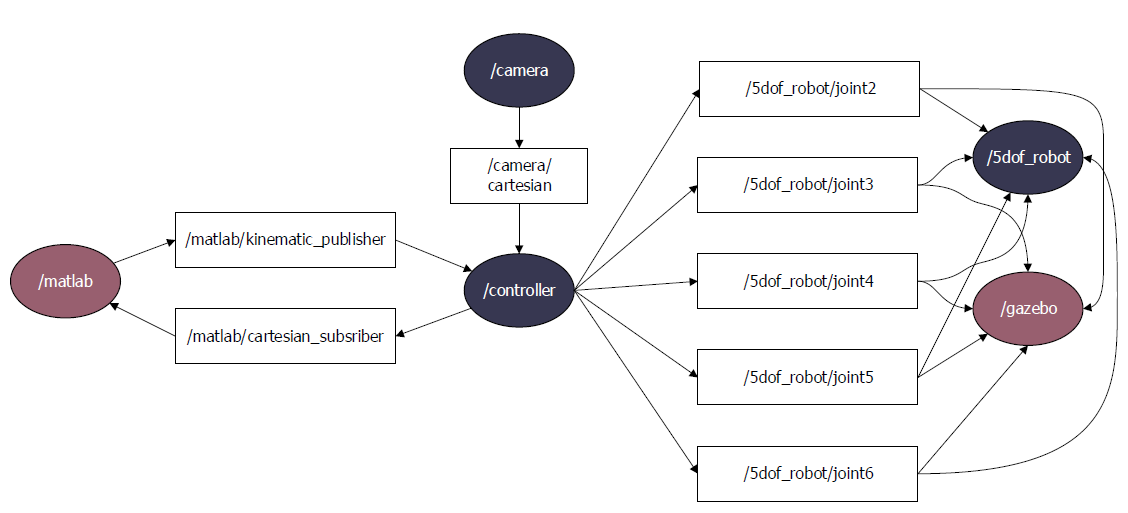
\includegraphics[width=\linewidth]{../Diagrams/NodeGraph-v1.png}
		\caption{Node graph}
		\label{fig:nodegraph}
	\end{figure}
	
	
	
	\subsection{Information flow}
	
	The flow of information in ARPA starts when the user sends a ready signal to the controller node. This signals that the controller will accept a Cartesian coordinate from the camera. This coordinate  further sent to MATLAB for processing. MATLAB returns five joints angles to the controller. These are the angles used to control both the physical arm and the Gazebo model. Hence, the controller publishes them to their respective topics, where they are picked up by both the Gazebo node and the 5DOF Robot node. After the control node has sent the joint angles, it waits for 5 seconds before it sends a new set of joint angles used to set the physical and simulated arm back to starting position. This process can be repeated by sending a new ready signal. Figure \ref{fig:seq-diagram} shows the flow of information in the form of a UML Sequence diagram.
	
	
	\begin{figure}[ht]
		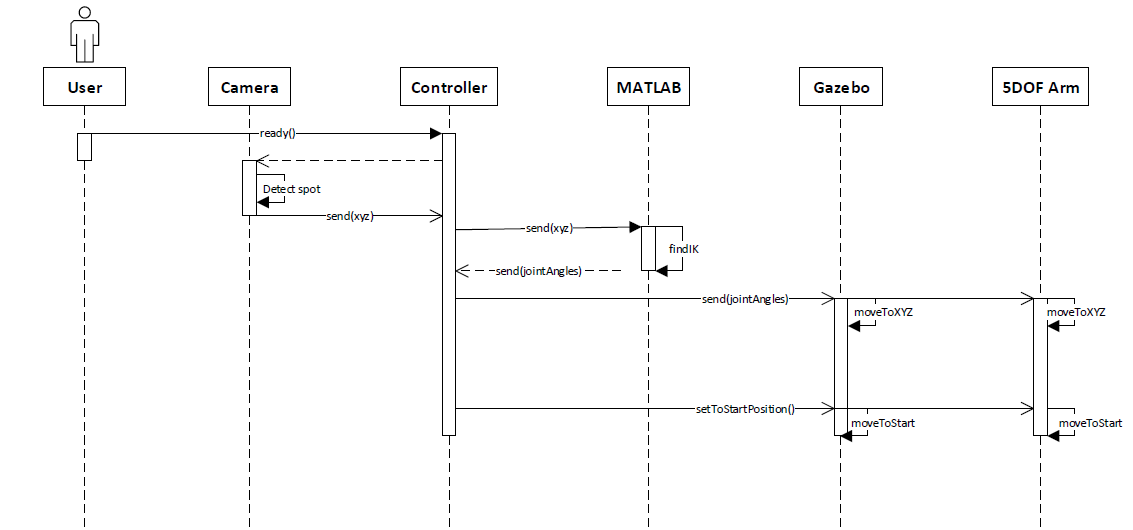
\includegraphics[width=\linewidth]{../Diagrams/SequenceDiagram-v1.png}
		\caption{UML Sequence diagram}
		\label{fig:seq-diagram}
	\end{figure}
	
	\subsection{Starting program}
	\label{startup}
	
	When running ARPA over two computers, one of them must be chosen to run as the ROS master. The selected master computer must source the master.sh script in every terminal used for running ROS commands. Next, the slave.sh script must be modified to contain the IP-address of the master computer. The address can be read from the output of the master.sh script. When the slave script is modified to contain the correct address, it must be sourced in all terminals on the slave computer that runs any ROS commands.
	
	Next up is to launch all ROS nodes. First of all, the setup.bash script in the devel directory of the catkin workspace must be sourced. When this is done on the master computer, the Arduino controlling the servos of the robotic arm must be connected to the computer. When it is connected, the command \textit{roslaunch robotic\_arm master.launch} can be run. Note that the launch file is configured to setup the ROS node on /dev/ttyACM0. This means that either the Arduino running the code must be connected before the Arduino used for power supply (see ), or the launch file must be modified to contain the correct device parameter. 
	
	The roslaunch command starts the camera, controller and the 5DOF robot node. The startup of the camera requires the user to set the coordinate system of ARPA's workspace. \textbf{todo: write calibration of camera}
	
	As with the master computer, the slave must also source the setup.bash script in the devel directory of the catkin workspace. When this is done, the command \textit{roslaunch simple\_robotic\_model joints.launch} can be run. This starts both the Gazebo and MATLAB node.
	
	\subsection{User interface}

	The user interface of ARPA is split into two: one on the master computer and one on the slave computer. Figure \ref{fig:ui-master} shows the user interface of the master. The window to the left is a live feed of the camera. It shows the user the detection of a red dot, i.e. where ARPA will move when given a ready signal. The window to the right allows the user to send this ready signal. When the ready.sh script is executed, the controller node will accept the next incoming coordinates and execute all necessary communications and actions for both the physical arm and the Gazebo model to move.
	
	\begin{figure}[ht]
		\centering
		\includegraphics[width=0.95\linewidth]{../Diagrams/UI-master.png}
		\caption{User interface: Master}
		\label{fig:ui-master}
	\end{figure}
	
	Figure \ref{fig:ui-slave} shows the user interface of the slave. Gazebo is launched as described in \textit{\ref{startup} Starting program}, but the rqt window on the left is not included as a part of the launch file. The user can choose to start rqt from a new terming through the \textit{rqt} command. The preferred setup for this project was to have rqt run the console plugin to show all the ROS messages in a GUI.
	
	\begin{figure}[ht]
		\centering
		\includegraphics[width=0.95\linewidth]{../Diagrams/UI-slave.png}
		\caption{User interface: Slave}
		\label{fig:ui-slave}
	\end{figure}
	
	\subsection{Dependencies}
	This section will summarize all the software dependencies used in the development of ARPA.
	\begin{itemize}
		\item \textbf{Ubuntu 16.04 LTS:} Operating System [http://releases.ubuntu.com/16.04.4/]
		\item \textbf{Robotic Operating System(ROS) Kinetic:} Framework for robot software [http://wiki.ros.org/kinetic/Installation/Ubuntu]
		\item \textbf{rosserial\_arduino:} Include Arduino into ROS node network [http://wiki.ros.org/rosserial\_arduino]
		\item \textbf{MATLAB:} Programming platform [https://se.mathworks.com/products/matlab.html]
		\item \textbf{Robotics System Toolbox:} MATLAB add-on providing different robotic software [https://se.mathworks.com/products/robotics.html]
		\item \textbf{OpenCV2:} Computer vision library [https://opencv.org/]
		\item \textbf{Python:} Programming language [https://www.python.org/]
	\end{itemize}
	
	\subsection{Hardware}
	During the project we had to make some adjustments to parts of the hardware related to the robotic arm. This section will go explain which adjustments has been made, and why.
	\subsubsection{Rig}
	When we were handed the robotic arm at the beginning of the course, we did some testing of it. First of all, we discovered that it had both had some loose screws, and also missing some. This lead us to spending some time on making the arm more rigid and secure. Figure \ref{fig:early-rig} shows this stage of the project.
	
	\begin{figure}[ht]
		\centering
		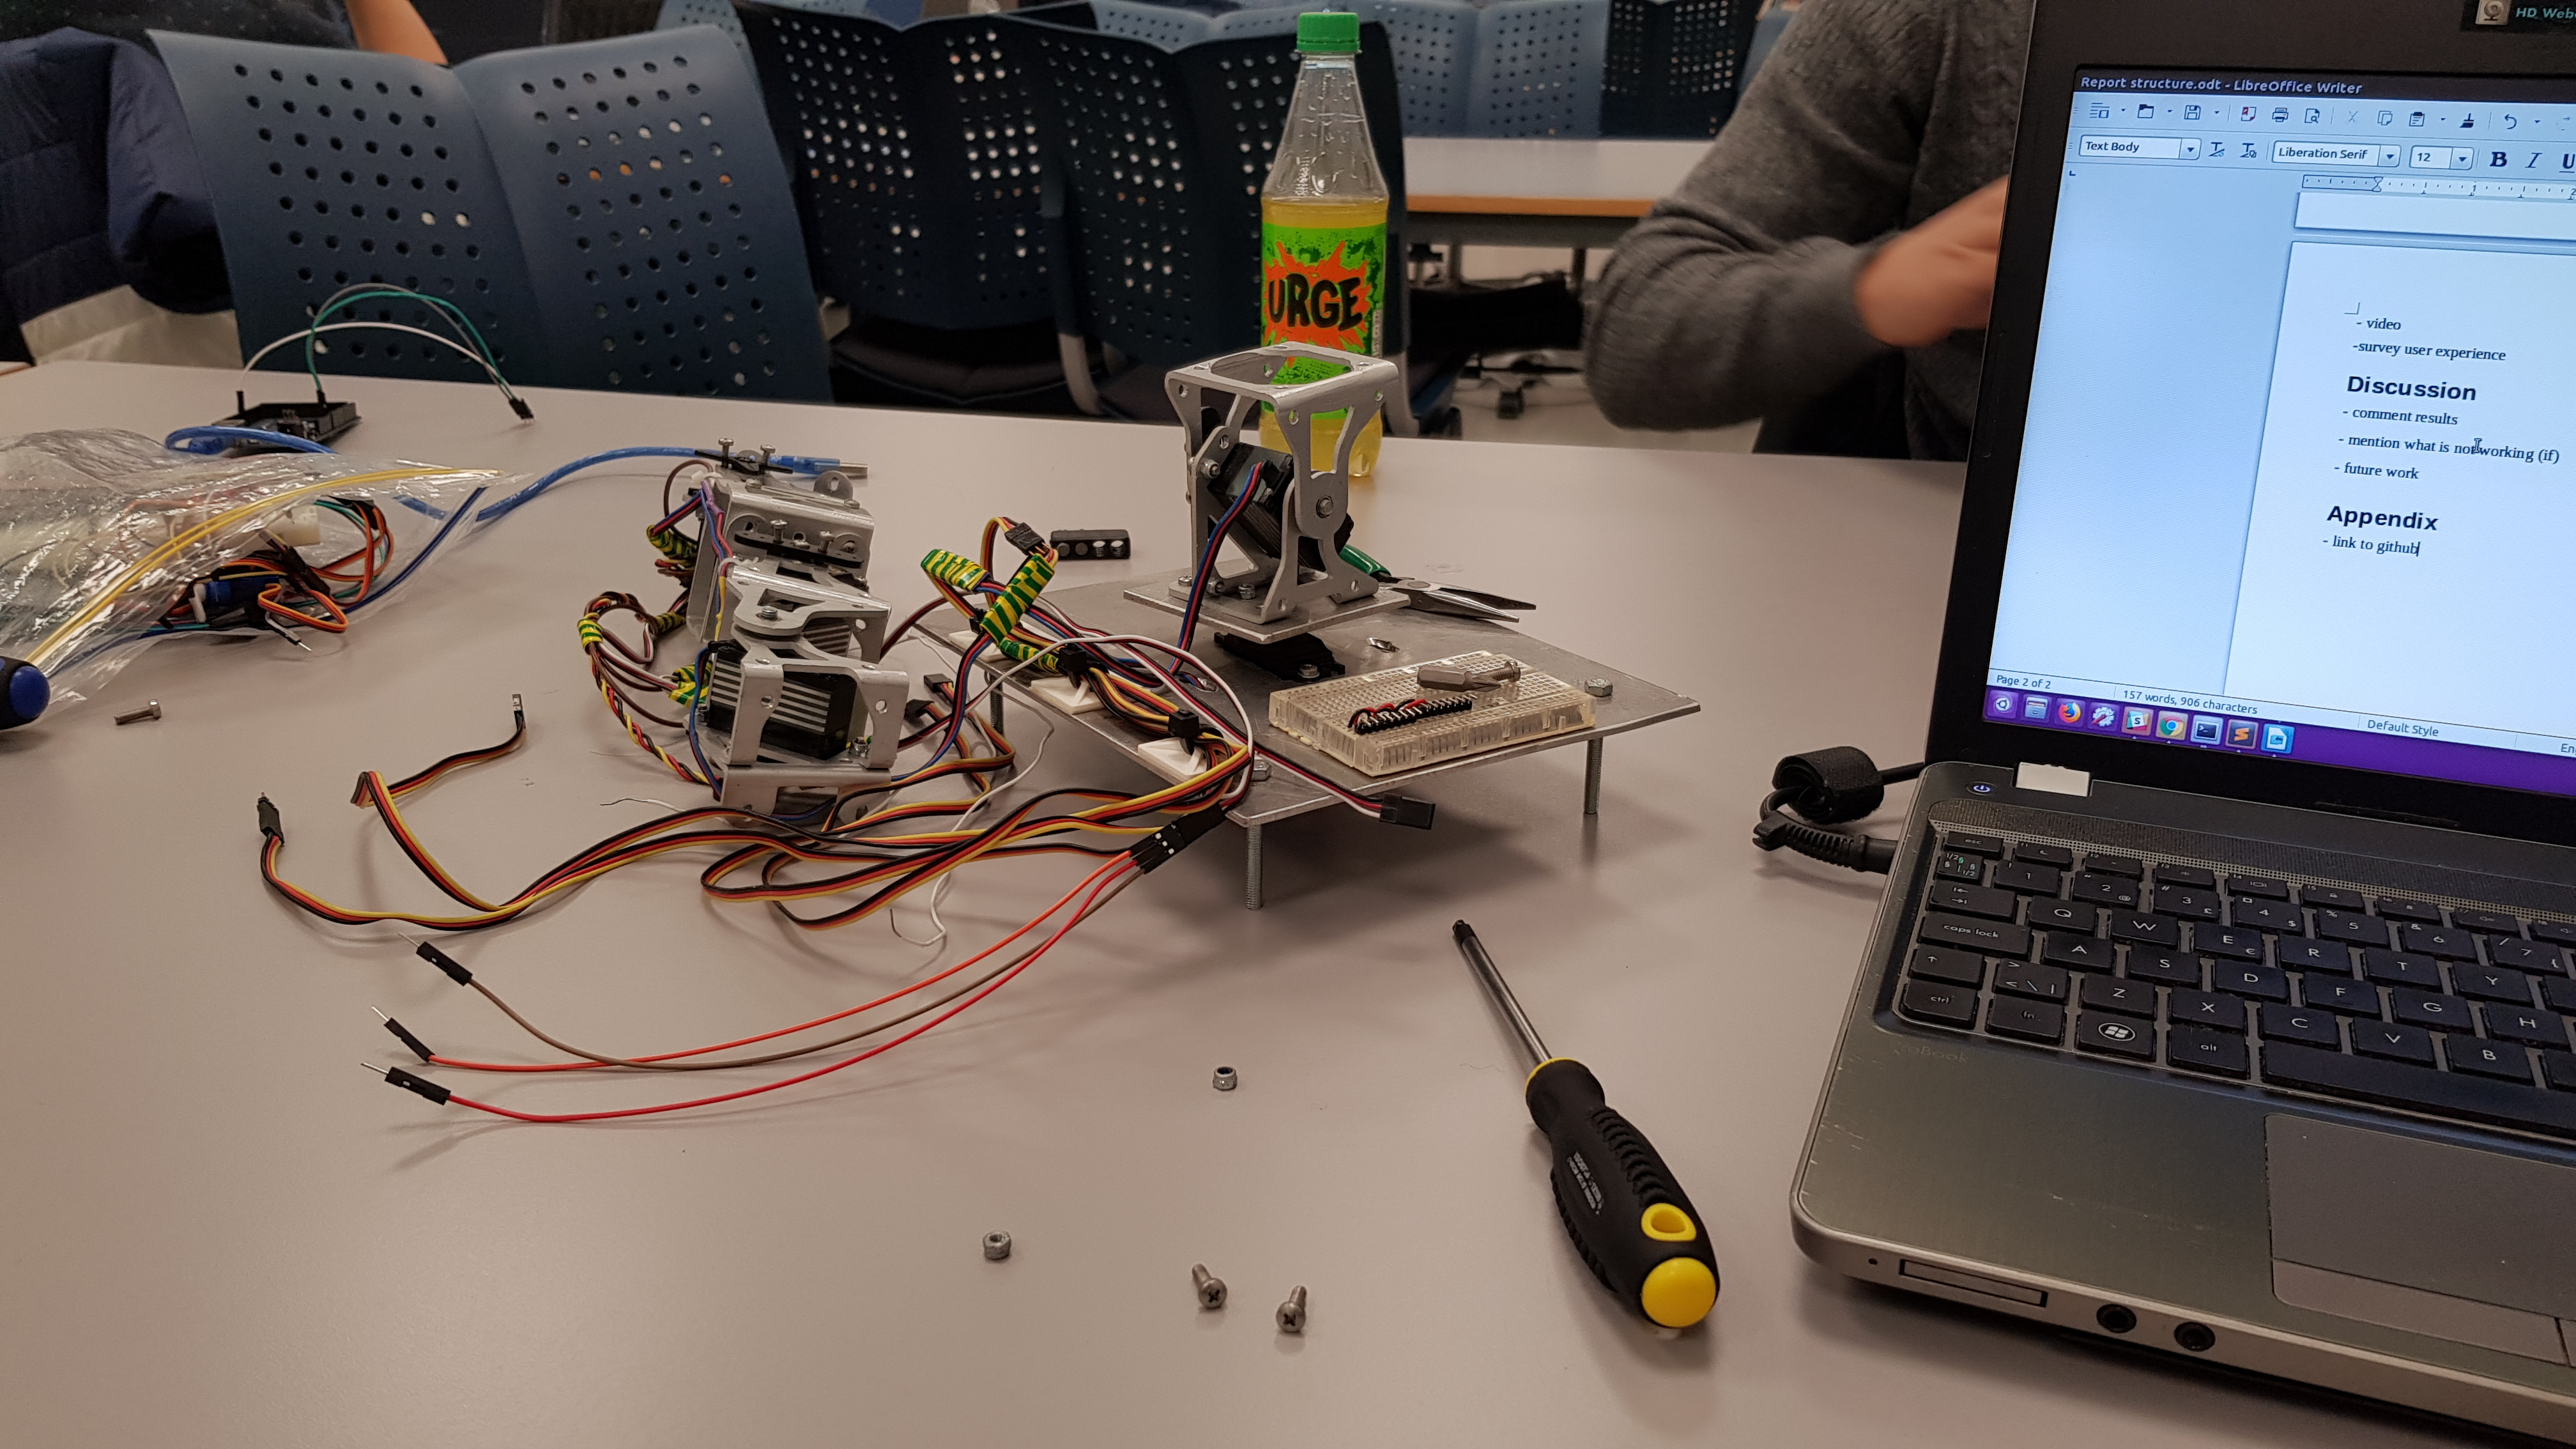
\includegraphics[width=0.8\linewidth]{../Diagrams/early-setup.jpg}
		\caption{Early stage of the hardware}
		\label{fig:early-rig}
	\end{figure}
	
	During the first tests of the robotic arm, we discovered that the torque would make the robot fall over. We decided to make a more stable mechanical rig, by attaching the robotic arm to a stable wooden rig. Figure \ref{fig:plank-rig} shows the process of making the wooden rig.
	
	\begin{figure}
	\centering
	
	
	\begin{subfigure}[t]{0.2\textwidth}
		
		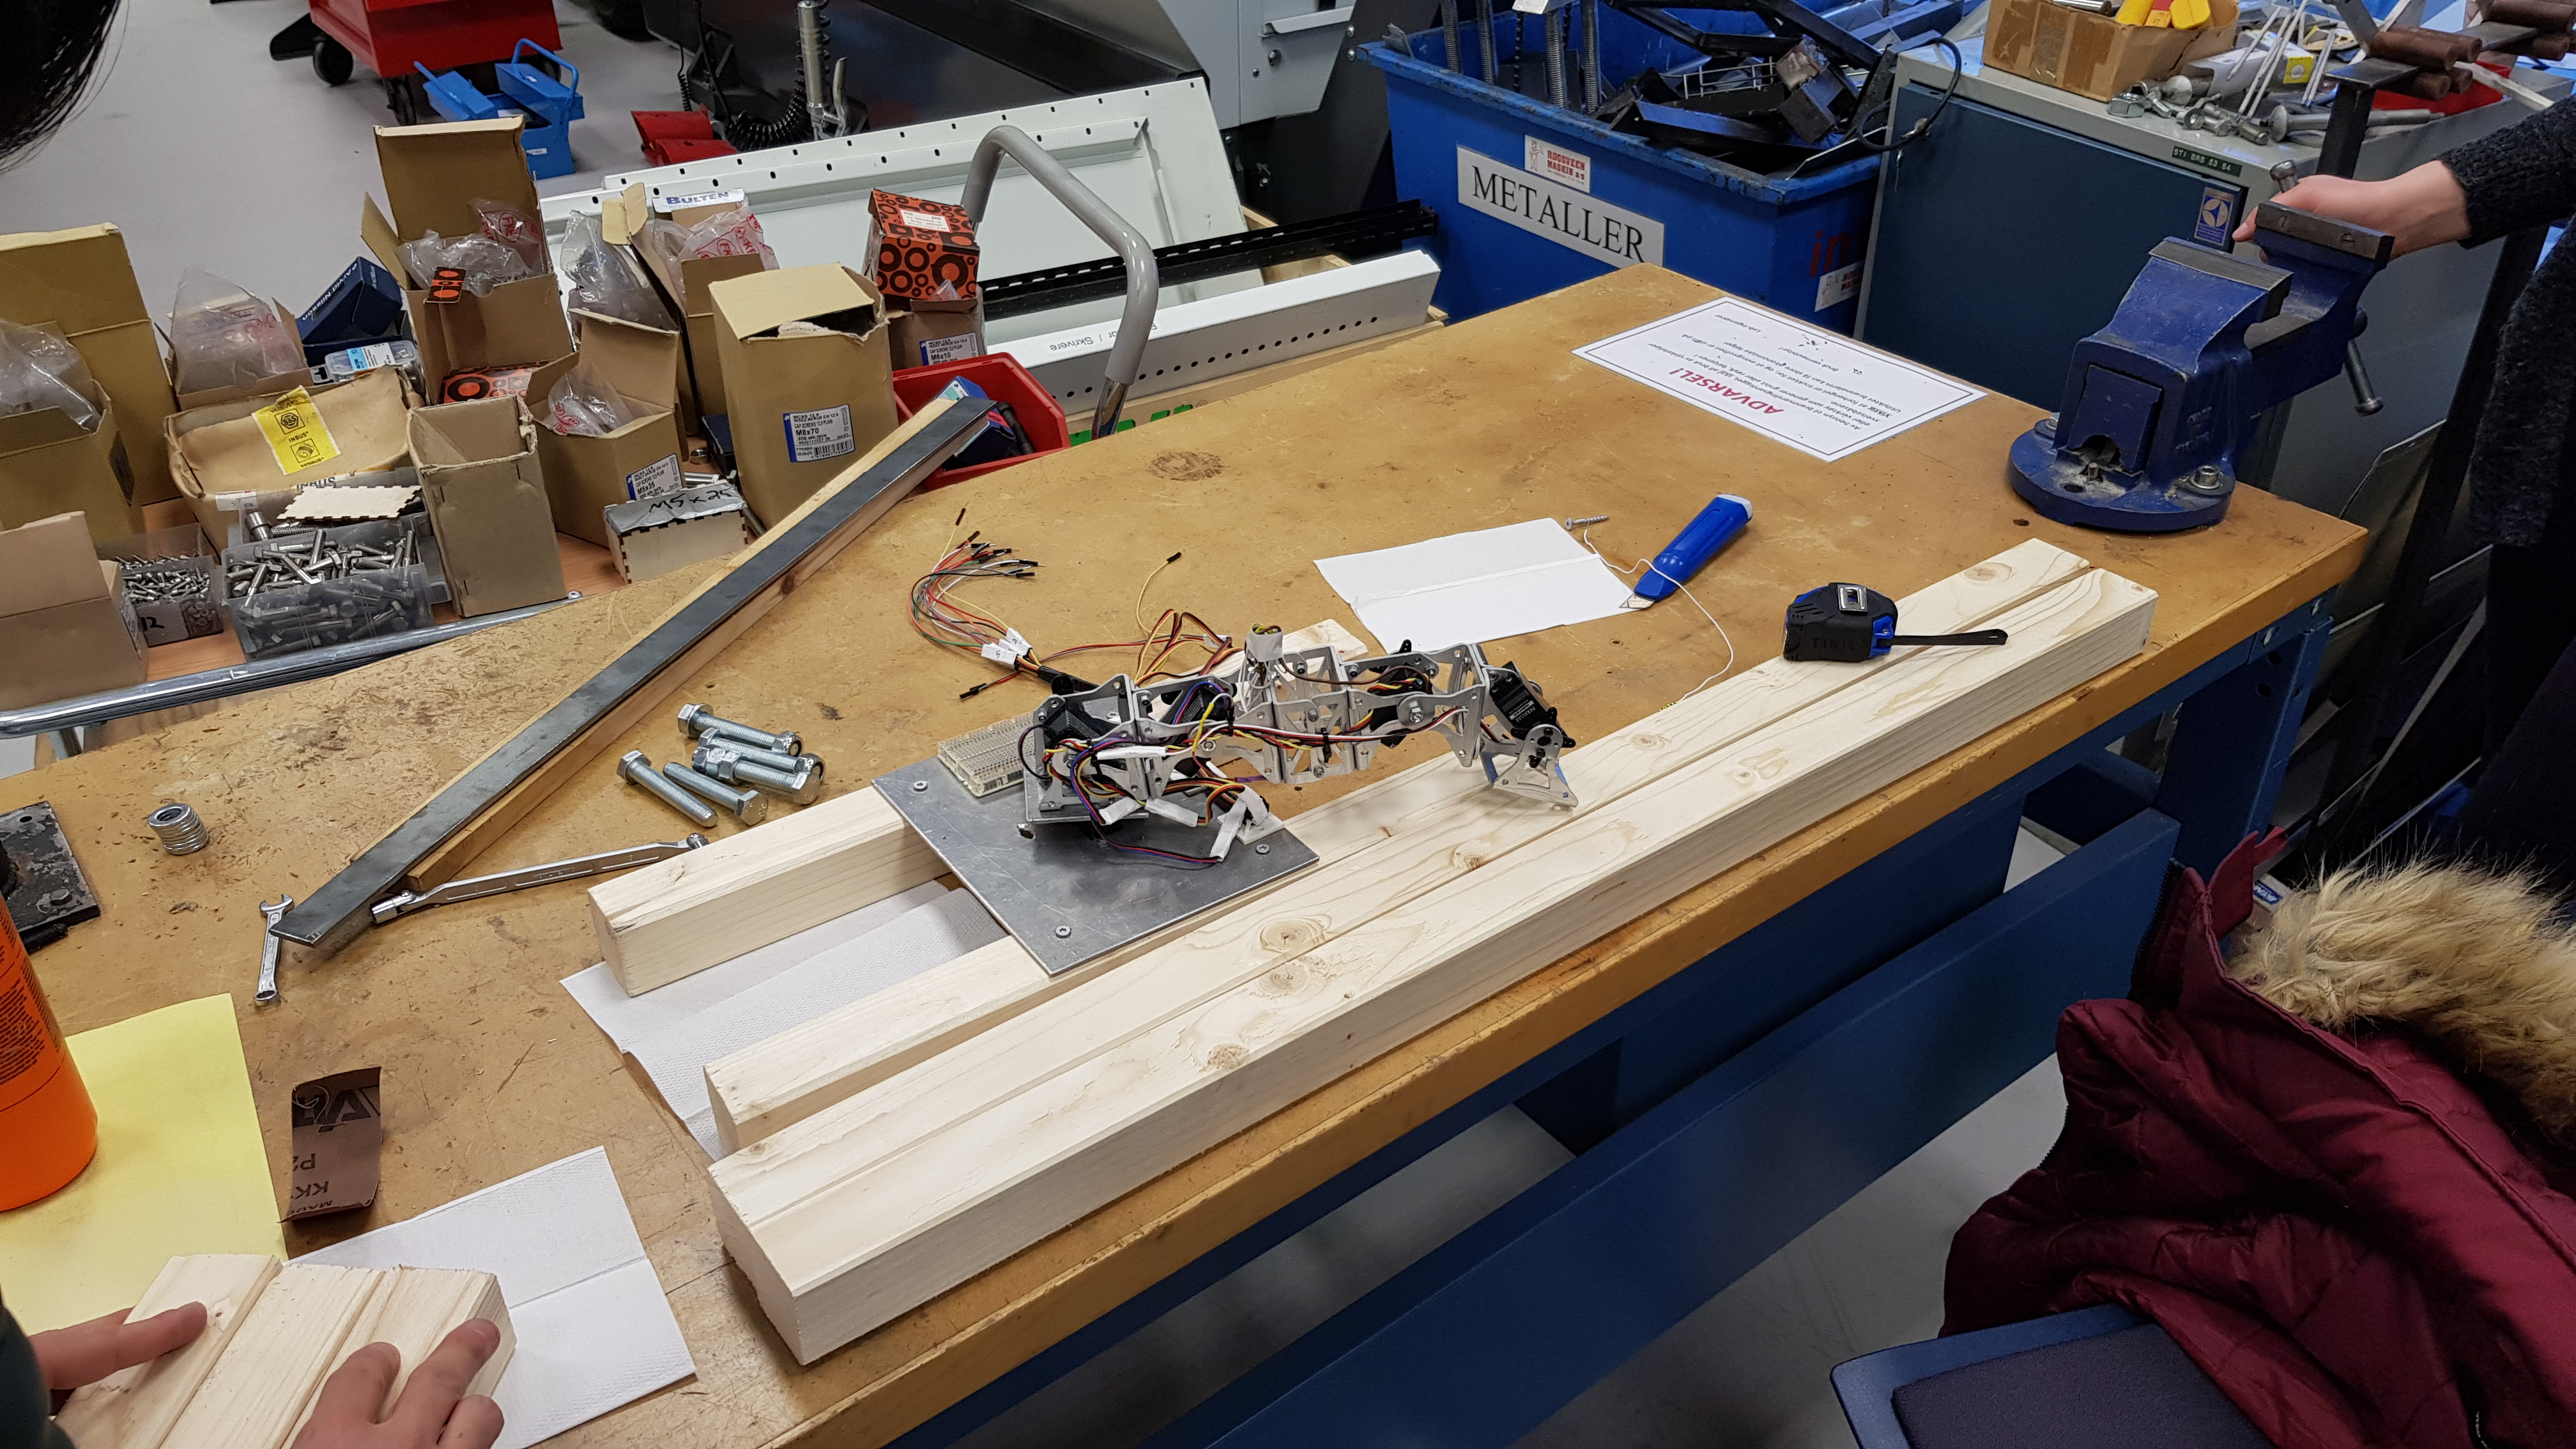
\includegraphics[height=1.2in]{../Diagrams/plank1.jpg}
		
		
	\end{subfigure}%
	
	\begin{subfigure}[t]{0.2\textwidth}
		\centering
		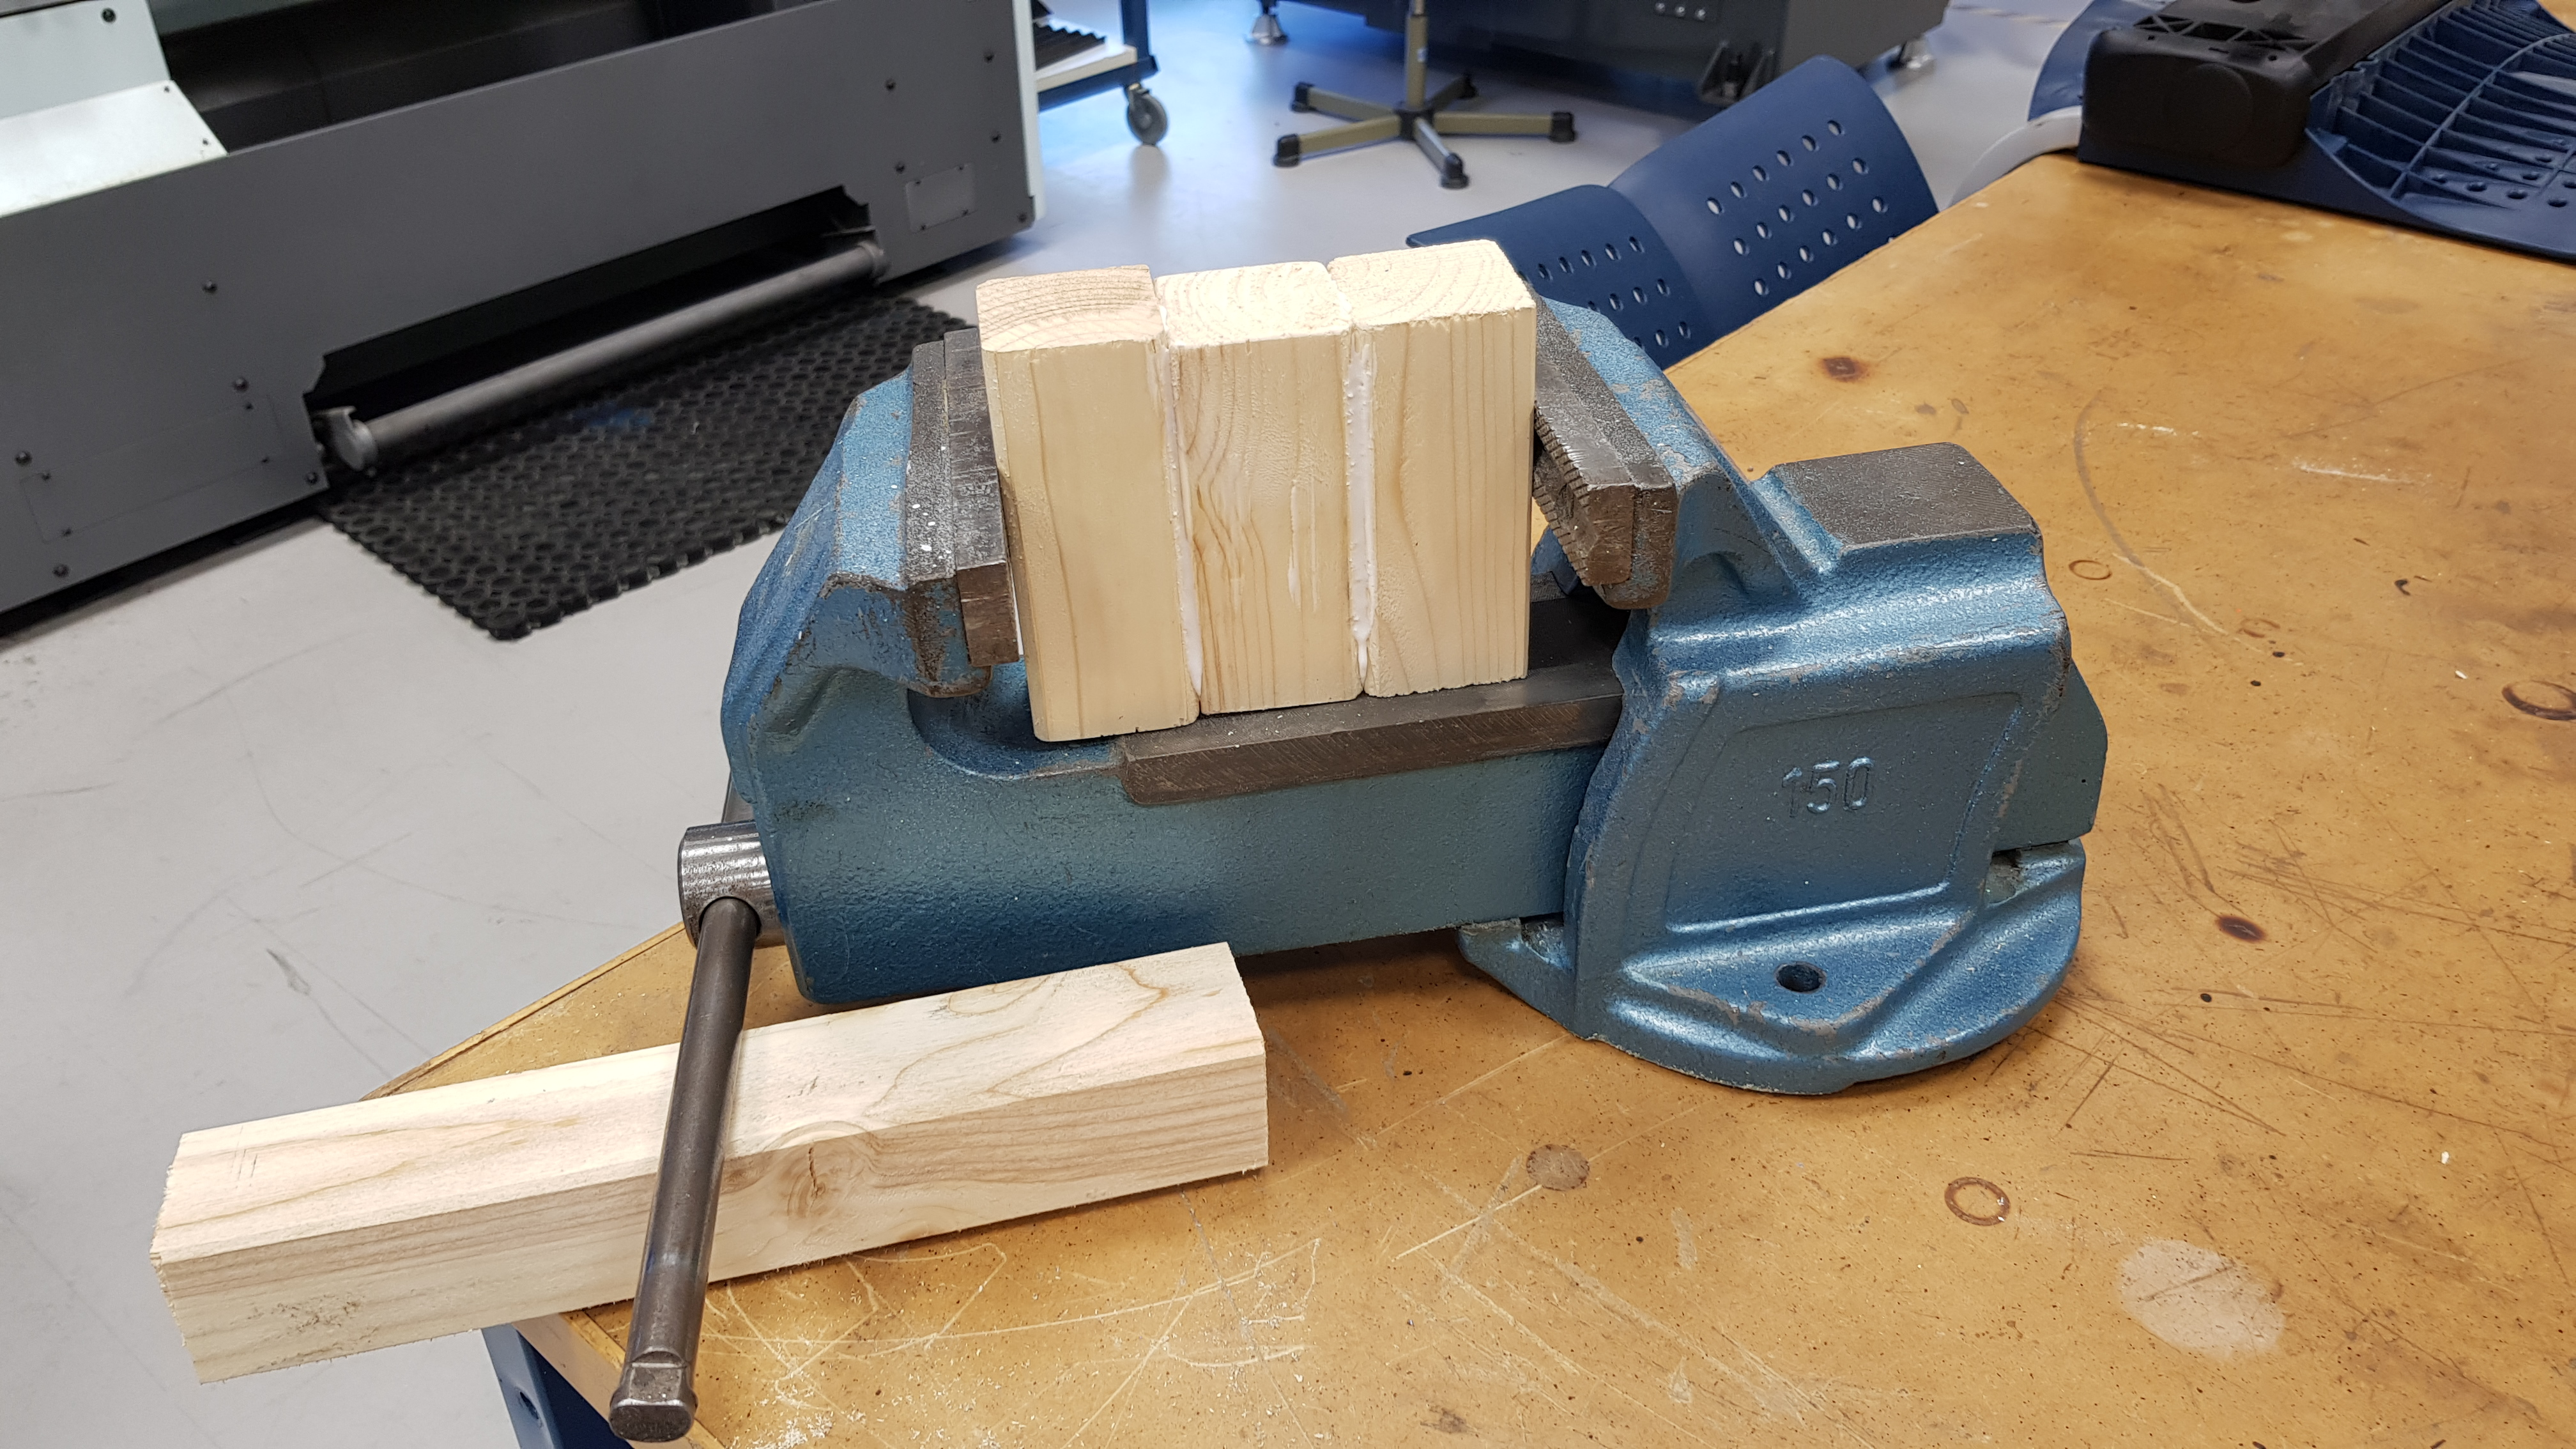
\includegraphics[height=1.2in]{../Diagrams/plank2.jpg}
		
	\end{subfigure}%
	
	\begin{subfigure}[t]{0.2\textwidth}
		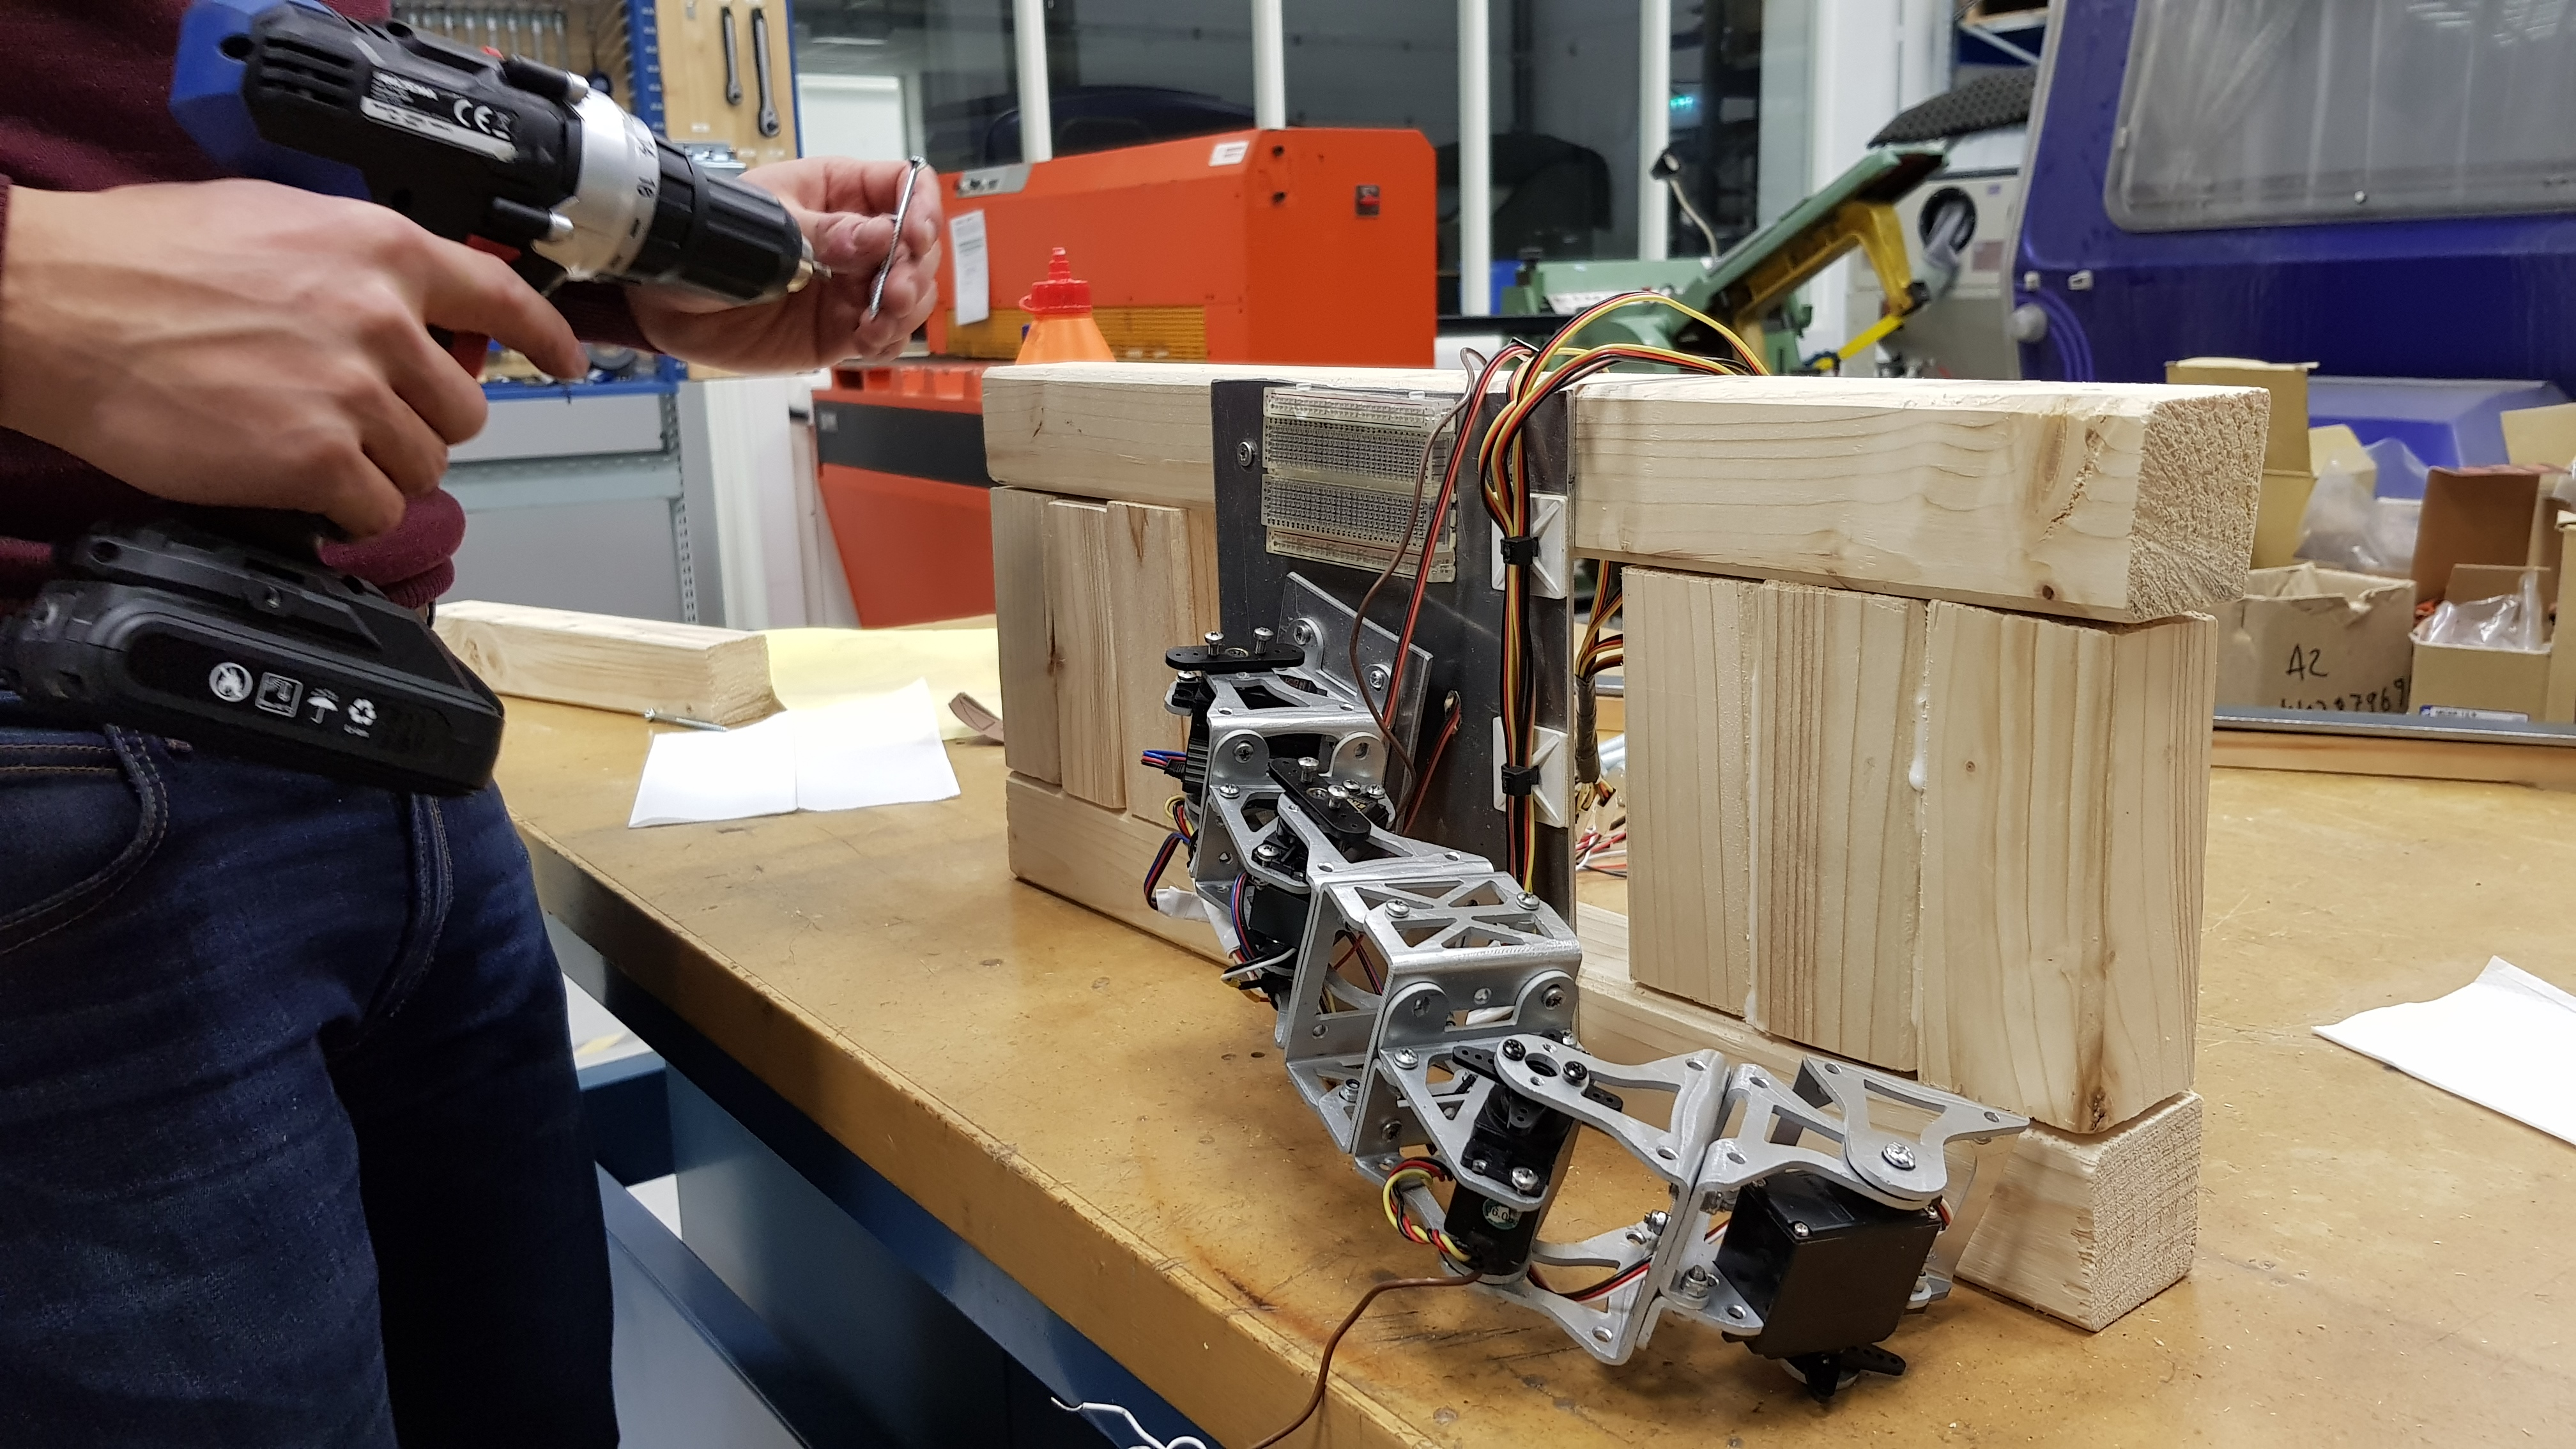
\includegraphics[height=1.2in]{../Diagrams/plank3.jpg}
		
	\end{subfigure}
	
	\begin{subfigure}[t]{0.2\textwidth}
		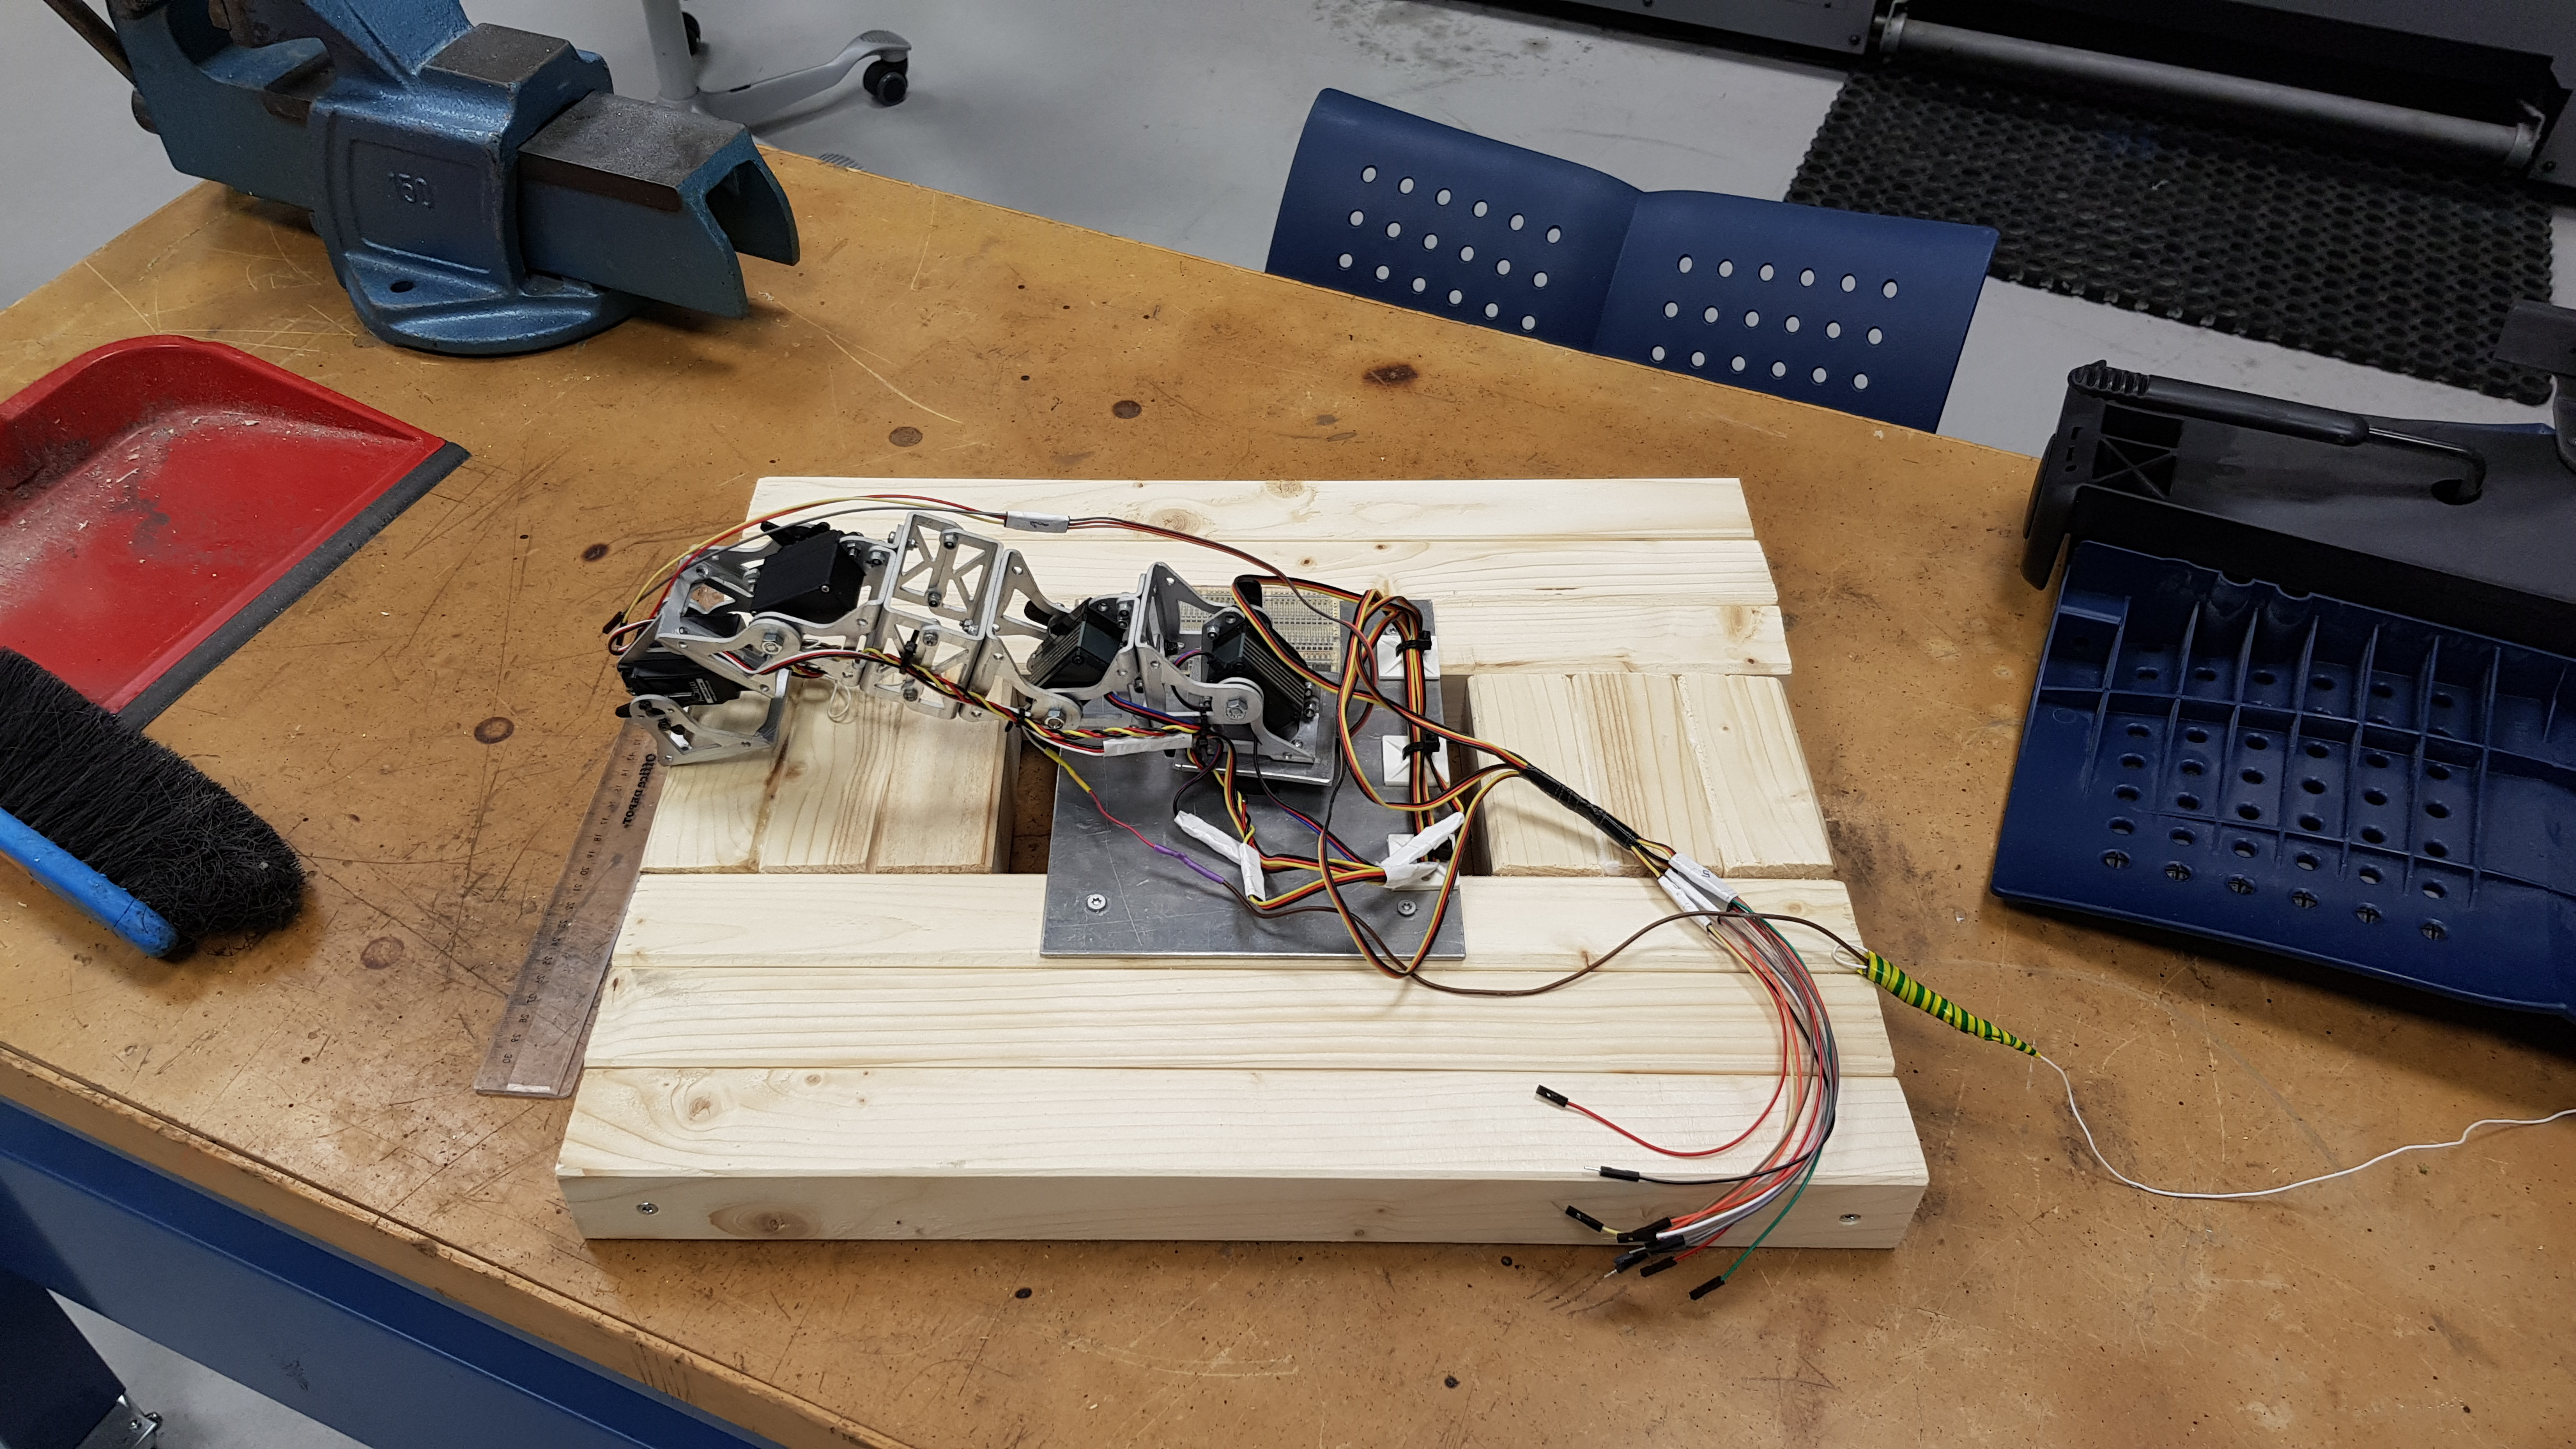
\includegraphics[height=1.2in]{../Diagrams/plank4.jpg}
		
	\end{subfigure}
	\caption{Process of making a wooden rig}
	\label{fig:plank-rig}	
	\end{figure}
	
	\subsubsection{Power supply}
	The servo motors are running nominally at 6V. As the arm consists of five motors, we could not power them all from the Arduino. We decided to buy battery holders to run 4 AA batteries in series. Since an AA battery is 1.5V, running four of them in series adds up to 6V.
	
	Due to the bigger torque on the bottom motors, we decided to supply the bottom three motors with 6V each,  having them run with nominal voltage level. The upper two motors of the arm are powered by one Arduino each, meaning they get 5V.
	
	
	
	%\section{Simulation and experiments}
	
	%\section{Discussion}
	
	%\section{Appendix}
	
	
\end{document}